
\section{Určenie typu zbrane}
Pre určenie typu zbrane v dvoch kategóriach a to na krátka a dlhé zbrane, boli navrhnuté dva klasické prístupy
    K-Nearest-Neighbor a SVM klasifikátor a dve architektúry pre konvolučné neurónové siete.

\subsection{Klasický prístup}
Pre trénovanie K-Nearest-Neighbor a SVM boli načítané všetky vstupné trénovancie dáta (1377 pre krátke zbrane a 850 pre dlhé zbrane),
    následne boli tieto dve skupiny zarovnané na rovnaký počet obrázkov pre každú kategórií na 850 obrázkov.
Následne bola veľkosť tejto vstupnej databázy, pomocou augmentácie dát, zväčšená štvornásobne a rozdelená na trénovacie a testovacie dáta.
Tieto augmentované dáta prešli predspracovaním ktoré pozostáva z normalizácie, šedotónovej, a hogovej transformácie.
Na trénovanie bolo použitých 5950 obrázkov, na testovanie resp. evaluáciu modelu 2550 obrázkov.

\subsubsection{SVM}
Trénovanie SVM klasifikátora prebiehalo so základnymi nastaveniami ktoré nastavuje scikit-learn knižnica pre triedu \textit{SVC}\footnote{\url{http://scikit-learn.org/stable/modules/generated/sklearn.svm.SVC.html}}.
Avšak pre porovnanie rôznych výsledkov bol pre dalšie trénovanie ešte zmenený kernel v SVM klasifikátore na ``linear''.

Štatistiky nižšie zobrazujú výsledky týchto dvoch SVM klasifikátorov, tabuľky vychádzaju z chybovej matice avšak
    zobrazujú ešte aj uspešnosť určenia v danej kategórií, ktorá je vyrátana ako
    $$uspesnost = \frac{spravne\_urcene}{spravne\_urcene + nespravne\_urcene} * 100$$
Výsledky ďalej ešte uvádzaju celkový výpočet úspešnosti.

\begin{table}[H]
    \centering
    \begin{tabular}{ccccc}
                                                                &                                    & \multicolumn{2}{c}{Klasifikované hodnoty}                                                         &                                    \\ \cline{3-5} 
                                                                & \multicolumn{1}{c|}{}              & \multicolumn{1}{c|}{Dlhé zbrane}                & \multicolumn{1}{c|}{Krátke zbrane}              & \multicolumn{1}{c|}{Úspešnosť}     \\ \cline{2-5} 
        \multicolumn{1}{c|}{}                                  & \multicolumn{1}{c|}{Dlhé zbrane}   & \multicolumn{1}{c|}{{\color[HTML]{009901} 761}} & \multicolumn{1}{c|}{{\color[HTML]{9A0000} 536}} & \multicolumn{1}{c|}{\textbf{61\%}} \\ \cline{2-5} 
        \multicolumn{1}{c|}{\multirow{-2}{*}{Správne hodnoty}} & \multicolumn{1}{c|}{Krátke zbrane} & \multicolumn{1}{c|}{{\color[HTML]{9A0000} 493}} & \multicolumn{1}{c|}{{\color[HTML]{009901} 760}} & \multicolumn{1}{c|}{\textbf{59\%}} \\ \cline{2-5} 
    \end{tabular}
    \caption{Výsledky klasifikácie pre SVM so základnymi nastaveniami.}
    \label{tab:svmrbf}
\end{table}
Celková úspešnosť je 59.65\% (viď. \ref{subsec:hodnoteniepresnosti}).

\begin{table}[H]
    \centering
    \begin{tabular}{ccccc}
                                                                &                                    & \multicolumn{2}{c}{Klasifikované hodnoty}                                                         &                                    \\ \cline{3-5} 
                                                                & \multicolumn{1}{c|}{}              & \multicolumn{1}{c|}{Dlhé zbrane}                & \multicolumn{1}{c|}{Krátke zbrane}              & \multicolumn{1}{c|}{Úspešnosť}     \\ \cline{2-5} 
        \multicolumn{1}{c|}{}                                  & \multicolumn{1}{c|}{Dlhé zbrane}   & \multicolumn{1}{c|}{{\color[HTML]{009901} 714}} & \multicolumn{1}{c|}{{\color[HTML]{9A0000} 540}} & \multicolumn{1}{c|}{\textbf{57\%}} \\ \cline{2-5} 
        \multicolumn{1}{c|}{\multirow{-2}{*}{Správne hodnoty}} & \multicolumn{1}{c|}{Krátke zbrane} & \multicolumn{1}{c|}{{\color[HTML]{9A0000} 498}} & \multicolumn{1}{c|}{{\color[HTML]{009901} 798}} & \multicolumn{1}{c|}{\textbf{62\%}} \\ \cline{2-5} 
    \end{tabular}
    \caption{Výsledky klasifikácie pre SVM s ``linear'' kernelom.}
    \label{tab:svmlinear}
\end{table}
Celková úspešnosť je 59.29\%.

\subsubsection{K-Nearest-Neighbor}
Trénovanie K-Nearest-Neighbor klasifikátora prebiehalo dvakrát, s prvým nastavením $k=5$, kde $k$ je celé číslo, ktoré určuje
    počet nabližších susedov na základne ktorých sa určuje kategória.
A s nastavením $k=1$.

\begin{table}[H]
    \centering
    \begin{tabular}{ccccc}
                                                                &                                    & \multicolumn{2}{c}{Klasifikované hodnoty}                                                         &                                    \\ \cline{3-5} 
                                                                & \multicolumn{1}{c|}{}              & \multicolumn{1}{c|}{Dlhé zbrane}                & \multicolumn{1}{c|}{Krátke zbrane}              & \multicolumn{1}{c|}{Úspešnosť}     \\ \cline{2-5} 
        \multicolumn{1}{c|}{}                                  & \multicolumn{1}{c|}{Dlhé zbrane}   & \multicolumn{1}{c|}{{\color[HTML]{009901} 880}} & \multicolumn{1}{c|}{{\color[HTML]{9A0000} 374}} & \multicolumn{1}{c|}{\textbf{70\%}} \\ \cline{2-5} 
        \multicolumn{1}{c|}{\multirow{-2}{*}{Správne hodnoty}} & \multicolumn{1}{c|}{Krátke zbrane} & \multicolumn{1}{c|}{{\color[HTML]{9A0000} 441}} & \multicolumn{1}{c|}{{\color[HTML]{009901} 885}} & \multicolumn{1}{c|}{\textbf{68\%}} \\ \cline{2-5} 
    \end{tabular}
    \caption{Výsledky klasifikácie pre K-Nearest-Neighbor s $k=5$.}
    \label{tab:kmeans5}
\end{table}
Celková úspešnosť je 69.22\%.

\begin{table}[H]
    \centering
    \begin{tabular}{ccccc}
                                                                &                                    & \multicolumn{2}{c}{Klasifikované hodnoty}                                                         &                                    \\ \cline{3-5} 
                                                                & \multicolumn{1}{c|}{}              & \multicolumn{1}{c|}{Dlhé zbrane}                & \multicolumn{1}{c|}{Krátke zbrane}              & \multicolumn{1}{c|}{Úspešnosť}     \\ \cline{2-5} 
        \multicolumn{1}{c|}{}                                  & \multicolumn{1}{c|}{Dlhé zbrane}   & \multicolumn{1}{c|}{{\color[HTML]{009901} 881}} & \multicolumn{1}{c|}{{\color[HTML]{9A0000} 373}} & \multicolumn{1}{c|}{\textbf{70\%}} \\ \cline{2-5} 
        \multicolumn{1}{c|}{\multirow{-2}{*}{Správne hodnoty}} & \multicolumn{1}{c|}{Krátke zbrane} & \multicolumn{1}{c|}{{\color[HTML]{9A0000} 405}} & \multicolumn{1}{c|}{{\color[HTML]{009901} 891}} & \multicolumn{1}{c|}{\textbf{69\%}} \\ \cline{2-5} 
    \end{tabular}
    \caption{Výsledky klasifikácie pre K-Nearest-Neighbor s $k=1$.}
    \label{tab:kmeans1}
\end{table}
Celková úspešnosť je 69.49\%.

\subsection{Konvolučné neurónové siete}
Pre určenie typu zbrane pomocou konvolučných neurónových sieti, boli použité dve navrhované architektúry (viď. \ref{subsec:navrharchitektur}).
Presné nastavenia a parametre siete boli popísane v návrhu.
Počet a rozdelenie vstupných dát na rovnaký pomer je totožný s uvedeným pri výsledkoch v klasickom prístupe, augmentácia dát
    prebiehala vždy počas každej epochy trénovania.
Celkovo bolo na trénovanie použitých 1190 obrázkov, na validáciu 255 a na testovanie tak isto 255 obrázkov.

\subsubsection{AlexNetLike}
Prvá archiktúra bola inšpirovaná AlexNet architektúrov, jej trénovanie prebiehalo v 40 epochách.
Kedže ako je vidno na obrázku \ref{pic:alexnetlikehistory}, medzi 30. a 40. epochou už veľké zlepšenie neprebiahlo, preto nebolo potrebné trénovať sieť ďalej.

\begin{figure}[H]
	\centering
	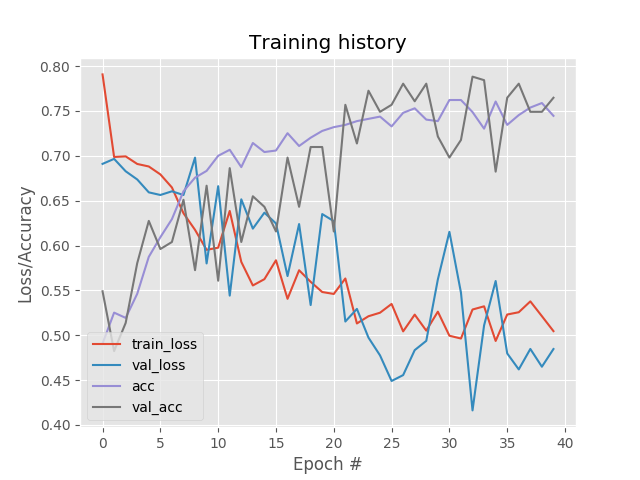
\includegraphics[width=0.75\textwidth]{alexnet-training_history}
	\caption{Priebeh trénovania siete AlexNetLike.}
	\label{pic:alexnetlikehistory}
\end{figure}
Kde \textit{acc} označuje celkovú presnosť siete na trénovacích dátach, \textit{val\_acc} presnosť siete na validačných dátach, \textit{train\_loss} a
    \textit{val\_loss} je tzv. \textit{loss\ function} alebo označovaná aj ako \textit{cost\ function}, ktorá v jednoduchosti určuje nepresnosť danej siete,
    to znamená že čím nižšia hodnota tým lepšia.

Výsledna presnosť na testovacích dátach je v tabuľke \ref{tab:alexnetresults}.

\begin{table}[H]
    \centering
    \begin{tabular}{ccccc}
                                                                &                                    & \multicolumn{2}{c}{Klasifikované hodnoty}                                                         &                                    \\ \cline{3-5} 
                                                                & \multicolumn{1}{c|}{}              & \multicolumn{1}{c|}{Dlhé zbrane}                & \multicolumn{1}{c|}{Krátke zbrane}              & \multicolumn{1}{c|}{Úspešnosť}     \\ \cline{2-5} 
        \multicolumn{1}{c|}{}                                  & \multicolumn{1}{c|}{Dlhé zbrane}   & \multicolumn{1}{c|}{{\color[HTML]{009901} 101}} & \multicolumn{1}{c|}{{\color[HTML]{9A0000} 23}}  & \multicolumn{1}{c|}{\textbf{81\%}} \\ \cline{2-5} 
        \multicolumn{1}{c|}{\multirow{-2}{*}{Správne hodnoty}} & \multicolumn{1}{c|}{Krátke zbrane} & \multicolumn{1}{c|}{{\color[HTML]{9A0000} 18}}  & \multicolumn{1}{c|}{{\color[HTML]{009901} 113}} & \multicolumn{1}{c|}{\textbf{86\%}} \\ \cline{2-5} 
    \end{tabular}
    \caption{Výsledky natrénovanej siete AlexNetLike.}
    \label{tab:alexnetresults}
\end{table}
Celková úspešnosť je 83.92\%.

\subsubsection{VGGLike}
Druhá architektúra bola inšpirovaná VGGLike architektúrov, jej trénovanie priebehalo tak isto v 40 epochách.

\begin{figure}[H]
	\centering
	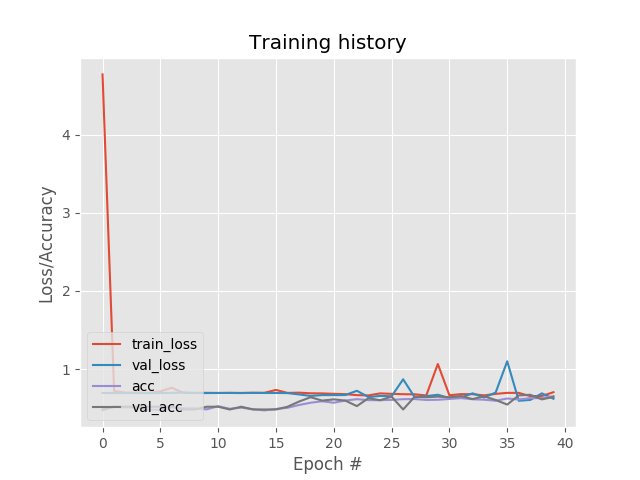
\includegraphics[width=0.75\textwidth]{vgglike-training_history}
	\caption{Priebeh trénovania siete VGGLike.}
	\label{pic:vgglikehistory}
\end{figure}

Počiatočná hodnota $train\_loss$ bola veľmi vysoká, graf je následkom toho veľmi skrekrelný a nieje možné presne vidieť postup trénovanie,
    avšak kompletné výsledky nad testovacími dátami sú uvedené v tabuľke \ref{tab:vgglikeresults}.

\begin{table}[H]
    \centering
    \begin{tabular}{ccccc}
                                                                &                                    & \multicolumn{2}{c}{Klasifikované hodnoty}                                                         &                                    \\ \cline{3-5} 
                                                                & \multicolumn{1}{c|}{}              & \multicolumn{1}{c|}{Dlhé zbrane}                & \multicolumn{1}{c|}{Krátke zbrane}              & \multicolumn{1}{c|}{Úspešnosť}     \\ \cline{2-5} 
        \multicolumn{1}{c|}{}                                  & \multicolumn{1}{c|}{Dlhé zbrane}   & \multicolumn{1}{c|}{{\color[HTML]{009901} 108}} & \multicolumn{1}{c|}{{\color[HTML]{9A0000} 26}}  & \multicolumn{1}{c|}{\textbf{87\%}} \\ \cline{2-5} 
        \multicolumn{1}{c|}{\multirow{-2}{*}{Správne hodnoty}} & \multicolumn{1}{c|}{Krátke zbrane} & \multicolumn{1}{c|}{{\color[HTML]{9A0000} 63}}  & \multicolumn{1}{c|}{{\color[HTML]{009901} 68}} & \multicolumn{1}{c|}{\textbf{48\%}} \\ \cline{2-5} 
    \end{tabular}
    \caption{Výsledky natrénovanej siete VGGLike.}
    \label{tab:vgglikeresults}
\end{table}
Celková presnosť siete je 67.06\%.
